\section{Der Modellbegriff}
\label{sec:Kap-3.1}

\vspace{-2mm} %%% für Druck

Der Begriff Modell ist in verschiedenen Disziplinen und Kontexten mit unterschiedlichen Bedeutungen belegt. Die wissenschaftlichen Modellbegriffe gehen aber alle mehr oder weniger stark auf die Arbeiten von Herbert Stachowiak zurück, der 1973 die „Allgemeine Modelltheorie“ \cite{sta73} veröffentlichte. Nach Stachowiak sind Modelle „Abbildungen [oder] Repräsentationen natürlicher oder künstlicher Originale, die selbst wieder Modelle sein können“ \cite[131]{sta73}. Über dieses sogenannte \textit{\mbox{Abbildungsmerkmal}} hinaus zeichnen sich Modelle nach Stachowiak dadurch aus, dass sie für einen spezifischen Adressaten(kreis) bestimmt sind, innerhalb bestimmter Zeit\-inter\-valle gültig sind und einen spezifischen Zweck verfolgen (\textit{Pragmatisches Merkmal}). Zudem erfassen Modelle nicht alle Merkmale ihres Originals, sondern nur diejenigen, die dem Ersteller des Modells für den Modellierungszweck relevant erscheinen (\textit{Verkürzungsmerkmal}). 

Ein Modell ist immer eine Abstraktion 
\marginline{Abstraktion}
des Originals. Das Original kann dabei bereits existieren, oder es soll noch erstellt werden. In der Softwareentwicklung ist meist Letzteres der Fall, ähnlich wie bei Modellen der Architektur (Hausbau, Brückenbau etc.). Abstraktion bedeutet, dass das Modell \textbf{keine vollständige} Darstellung des Originals ist. Zum einen wird es nur diejenigen Aspekte des Originals beinhalten, die dem Ersteller des Modells für den vorgesehenen Einsatz des Modells zweckmäßig erschienen. Zum anderen beinhaltet Abstraktion die Möglichkeit, dass Eigenschaften des Originals in einem geringeren Detaillierungsgrad als im Original dargestellt werden können. So könnte ein Modell eines Softwareprodukts zum Beispiel auf einer hohen Abstraktionsebene nur die großen Komponenten darstellen. Auf einer niedrigeren Abstraktionsebene könnte ein anderes Modell desselben Softwareprodukts jedes einzelne Softwareobjekt zeigen. Die Wahl einer geeigneten Abstraktionsebene für ein Modell ist neben den Punkten Einsatzzweck und Zielgruppe ein entscheidender Faktor für die Nützlichkeit des Modells. In diesem Zusammenhang sei erwähnt, dass im Softwareengineering ein konkretes Modell in der Regel nicht richtig oder falsch ist – wie es in Disziplinen oder Bereichen sein kann, in denen der Modell\-begriff stark mit dem Begriff der Theorie verknüpft ist. Es ist nur für die anvisierte Zielgruppe und den Einsatzzweck mehr oder weniger nützlich.

Im Softwareengineering werden Modelle in unterschiedlichen Situationen eingesetzt. Abbildung~\ref{fig:modellbegriff_softwareengineering} zeigt unter Rückgriff auf Stachowiaks allgemeinen Modellbegriff einen Modellbegriff für das Softwareengineering und seine verschiedenen Ebenen.

% Die Grafik ist breiter als die Textbreite.
\begin{figure}[t]
	\begin{addmargin*}[0cm]{-\marginparwidth}
	\begin{addmargin*}[0cm]{-\marginparsep}
		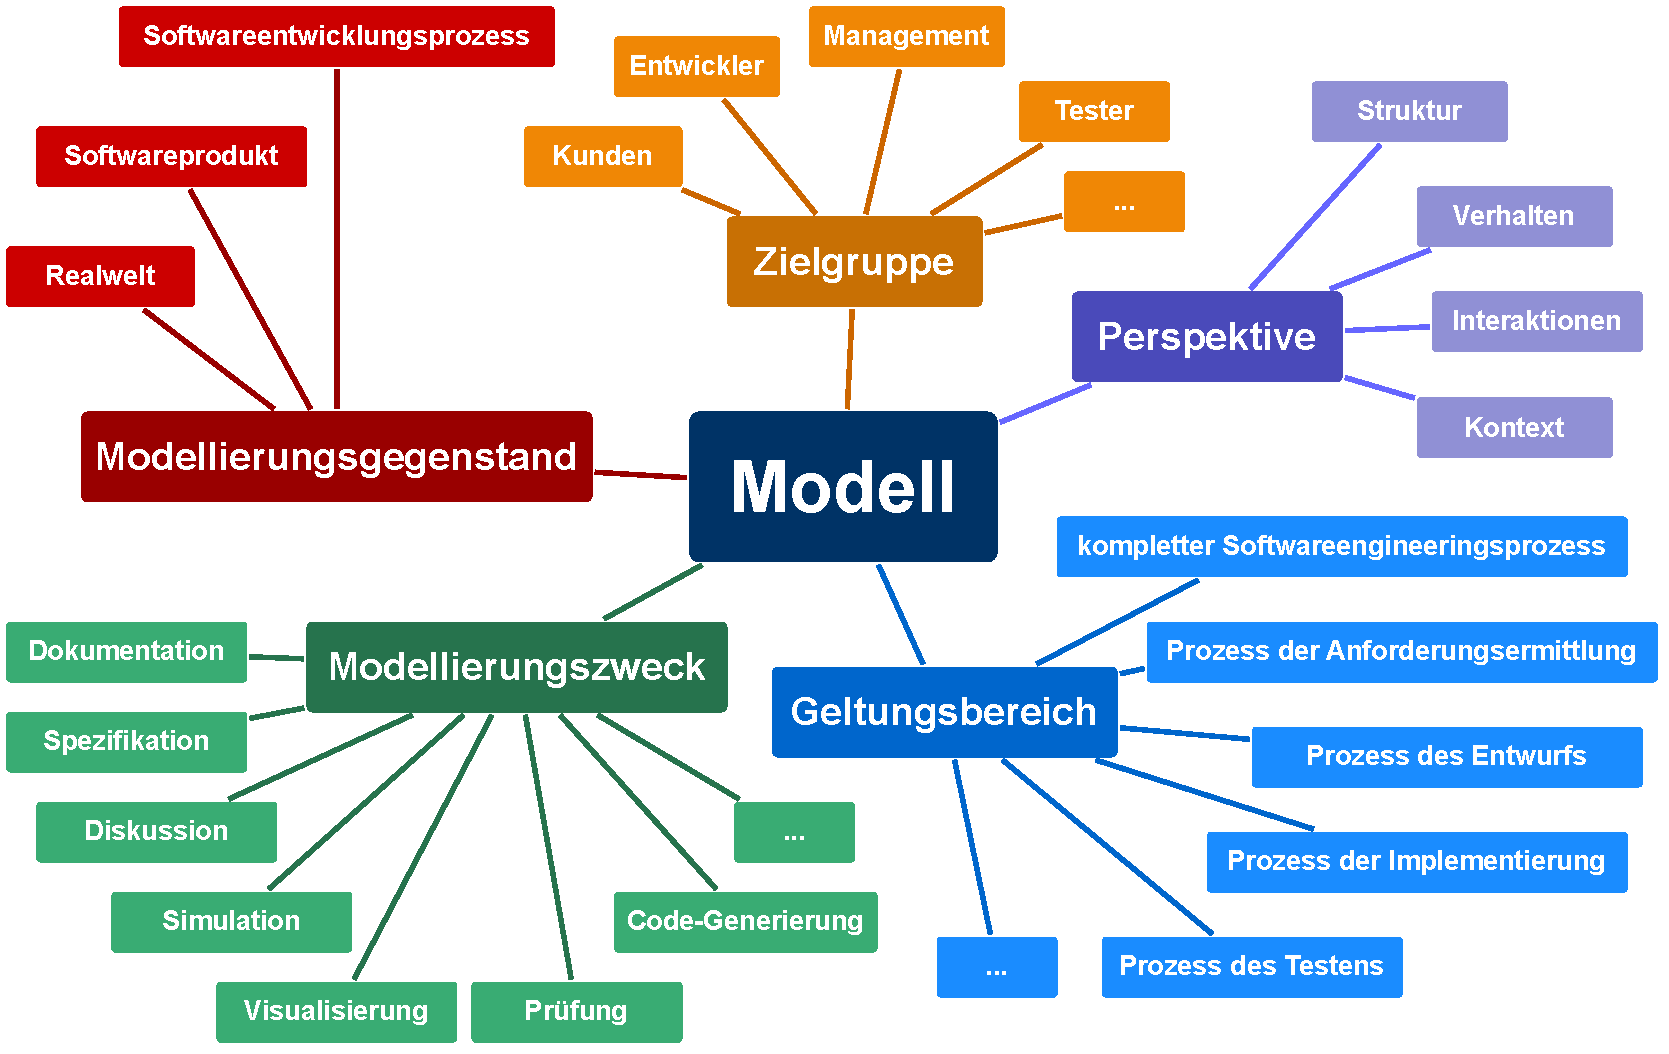
\includegraphics[scale=0.62]{Bilder/Kapitel-3/Abb-3-1-MindMap.pdf}
		\caption{Modellbegriff fürs Softwareengineering}
		\label{fig:modellbegriff_softwareengineering}
	\end{addmargin*}
	\end{addmargin*}
\end{figure}		

\vspace{1mm} % Ausgleich für den farblichen Kasten

\sttpMindMapText[colMindMap1]{\textbf{\textsf{Modellierungsgegenstand}}}
von Modellen können Softwareentwicklungsprozesse sein. Vertreter solcher Modelle haben Sie in Kapitel 2 %~\ref{sec:Kap-2}
mit den Vorgehensmodellen schon kennengelernt. Anstelle des Entwicklungsprozesses kann der Modellierungs\-gegenstand aber auch ein (zu entwickelndes) Softwareprodukt sein. In dieser Lektion werden Sie erstmalig Modelle kennenlernen, mit denen die \textbf{Realwelt} – bzw. genauer: der für die Entwicklung des Softwareprodukts relevante Ausschnitt der Realwelt, die sogenannte Domäne – abgebildet werden kann.

Eine weitere Ebene eines Softwareengineering-Modells ist die vom Modell eingenommene
\sttpMindMapText[colMindMap2]{\textbf{\textsf{Perspektive}}}
auf den Modellierungsgegenstand. Ein Modell kann die Struktur (\zb Aufbau, Elemente, statische Beziehungen zwischen Elementen) des Model\-lie\-rungs\-gegen\-stands zeigen, aber auch sein Verhalten (\zb Antwortverhalten auf \mbox{Ereignisse}) oder seine Interaktionen (zwischen verschiedenen Komponenten oder mit der Umgebung). Oder der Blickwinkel eines Modells ist auf die Abgrenzung zwischen dem Modellierungsgegenstand und seiner Umgebung gerichtet (die Perspektive Kontext in der Abbildung). Die aus Kapitel 2 %~\ref{sec:Kap-2}
bekannten Vorgehensmodelle betrachten in erster Linie die Struktur von Softwareentwicklungsprozessen und die Interaktion zwischen deren Komponenten, also den einzelnen Prozessen des Softwareengineering. 

\vspace{1mm} % Ausgleich für den farblichen Kasten

Der 
\sttpMindMapText[colMindMap3]{\textbf{\textsf{Geltungsbereich}}}
eines Vorgehensmodells ist meistens der komplette Softwareentwicklungsprozess. Andere Modelle im Softwareengineering, deren Modellierungsgegenstände ebenfalls Softwareentwicklungsprozesse sind, fokussieren sich nur auf bestimmte Teile dieses Softwareentwicklungsprozesses, zum Beispiel wenn sie nur den Prozess der Anforderungsermittlung im Blick haben. Für solche Modelle wird in Abgrenzung zum Begriff Vorgehensmodell häufig der Begriff \textit{Methode} verwendet – wobei der Begriff Methode in diesem Kontext nicht mit dem Begriff der Methode aus dem Kontext der Programmierung verwechselt werden darf. Der Begriff Methode ist im Softwareengineering sehr weit gefasst: Darunter fallen Konzepte, Para\-digmen, Strategien, Verfahren, Richtlinien oder sonstige Arten von Anleitungen, deren Ziel eine systematische Entwicklung von Software ist. So kann man sowohl die strukturierte Programmierung aus Abschnitt~1.1 %~\ref{sec:Kap-1.1}
als auch die Erhebung von Anforderungen mit Hilfe von Anwendungsfällen als Methode bezeichnen. In der Literatur wird auch Extreme Programming manchmal als Methode anstatt als Vorgehensmodell bezeichnet. Die Grenze zwischen Vorgehensmodell und Methode ist nicht immer eindeutig zu ziehen, insbesondere wenn sich ein Ansatz auf mehrere Prozesse des Softwareengineering bezieht. Letztendlich ist die Abgrenzung aber auch nur insofern relevant, dass man sowohl im Kapitel zu Methoden als auch im Kapitel zu Vorgehensmodellen eines Softwareengineering-Buchs suchen sollte, wenn man einen bestimmten Ansatz recherchieren möchte.

Im Softwareengineering werden zu einem Modellierungsgegenstand in der Regel mehrere Modelle erstellt. Durch unterschiedlich gewählte Abstraktionsebenen und unter\-schied\-liche Blickwinkel können schrittweise gezielt bestimmte Aspekte des abzu\-bildenden oder zu erstellenden Originals (Produkt, Prozess, Realwelt) untersucht werden und dabei jeweils Anforderungen oder Probleme des Gesamtkomplexes ausgeblendet werden. Insofern helfen Modelle bei der Verringerung von Komplexität – ein auf den verschiedensten Ebenen ganz zentrales Thema in der Software\-entwicklung. 

Außerordentlich wichtig 
bei der Erstellung jedes Modells sind die
\sttpMindMapText[colMindMap4]{\textbf{\textsf{Zielgruppe}}}
des Modells und der 
\sttpMindMapText[colMindMap5]{\textbf{\textsf{Modellierungszweck}}}. Die Kombination beider Faktoren bestimmt die konkrete Ausgestaltung des Modells. So wird zum Beispiel ein vom Entwicklungsleiter erstelltes Modell zur Diskussion mit dem Kunden über das Verhalten eines geplanten Softwareinkrements anders aussehen als das von derselben Person erstellte Modell für die gleiche Diskussion mit seinem Entwicklungsteam. Ebenso wird sich das Modell für den Kunden, das zu Diskussionszwecken erstellt wurde, von dem Modell für denselben Kunden unterscheiden, das zur Dokumentation der getroffenen Entscheidungen erstellt wird. Neben den in der Abbildung aufgeführten Zielgruppen und Modellierungszwecken sind viele weitere Gruppen und Zwecke denkbar. 

\sttpDefinitionskasten{\sttpDefinitionskastenSkalierungsfaktor}{Modell im Softwareengineering}{Die Abstraktion eines Originals, die für eine bestimmte Zielgruppe geschaffen wurde, einen definierten Einsatzzweck besitzt und eine spezifische Perspektive auf das Original einnimmt. Der Geltungsbereich des Modells kann der komplette Softwareentwicklungsprozess sein oder Teile davon.} 

\minisec{Modelle darstellen}
\phantomsection
\label{sec:Kap-3.1:Modelle_darstellen}
Damit man überhaupt mit Modellen arbeiten kann (über sie diskutieren, sie als Doku\-men\-ta\-tion verwenden etc.), müssen sie in irgendeiner Weise sichtbar sein. Das bedeutet, man benötigt Darstellungsmittel für Modelle. Im Rahmen des Softwareengineering werden Modelle häufig in Form von grafischen Notationen (Diagrammen) aufgeschrieben. Eine Notation ist eine Sammlung von (textuellen oder grafischen) Zeichen und Symbolen, die bestimmte Gegenstände oder Konzepte repräsentieren. Im Softwareengineering wird weitgehend synonym zum Begriff der Notation der Begriff der
\marginline{Modellierungs\-sprache}
\textit{Modellierungs\-sprache} verwendet. Modellierungssprachen legen einen Satz von Regeln fest, der bestimmten Elementen, zum Beispiel Kästchen oder \mbox{Pfeilen} einer bestimmten Form innerhalb eines Diagramms, eine jeweilige Bedeutung zuweist. Diese grafischen Darstellungen können um textuelle Darstellungen – in Form von Prosa oder in von der Modellierungssprache vorgegebener, stärker formularhafter Form – ergänzt werden. Die in diesem Text thematisierte Unified Modeling Language ist eine überwiegend grafische Modellierungssprache, die für verschiedene Zwecke aber auch textuelle Ergänzungen zu den Diagrammen anbietet. 

Neben den grafischen Modellierungssprachen werden im Softwareengineering auch rein textuelle Modellierungssprachen sowie formal-mathematische Notationen eingesetzt – allerdings deutlich seltener. Eine formalere Darstellung von Modellen anstelle der Diagrammdarstellung ist vor allem zu zwei Einsatzzwecken notwendig: Wenn aus im Rahmen der Softwareentwicklung erstellten Modellen automatisiert verfeinerte Modelle oder sogar Programmcode des zukünftigen Softwareprodukts erzeugt werden sollen, reichen grafische Diagramme nicht aus. Der zweite Einsatzzweck ist die formale Spezifikation – und damit auch mögliche formale Prüfung – von Anforderungen im Rahmen der Anforderungsermittlung und -analyse. 

Modelle im objektorientierten Softwareengineering setzen sich oft aus Submodellen zusammen. Jedes Submodell erfüllt seinen eigenen Zweck, indem es einen anderen Teil des Originals betrachtet oder einen anderen Blickwinkel einnimmt als ein anderes Submodell. Der  Begriff Modell 
\marginline{Modell und Diagramm}
und insbesondere die Abgrenzung zwischen den Begriffen Modell, Submodell und Diagramm wird in der Literatur uneinheitlich gehandhabt. Wir verfahren in diesem Kontext pragmatisch: Zum einen ist für uns ein Submodell gleichwertig mit einem Modell. So sind ein Strukturmodell und ein Verhaltensmodell zum selben Original einfach zwei Modelle, unabhängig davon, ob sie zusammen eingesetzt werden – und damit im strengen Sinne zwei Submodelle eines Gesamtmodells bilden würden – oder unabhängig voneinander das Original aus dem jeweiligen spezifischen Blickwinkel beschreiben.  Zum anderen gilt für die Beziehung zwischen Modell und Diagramm: Ein Diagramm (inklusive eventueller textueller Ergänzungen) bzw. eine Kombination aus mehreren Diagrammen \textbf{ist} die Manifestation eines Modells. Insofern wird in diesem Text beides als gleichbedeutend betrachtet. Wenn ein Diagramm verändert wird (\zb Elemente ergänzt oder Aspekte verfeinert) oder eine Menge zusammengehöriger Diagramme um ein weiteres Diagramm erweitert wird, entsteht ein neues Modell. 
